\documentclass[compress,]{beamer}

%loading packages
\usepackage[ngerman]{babel}
\usepackage[T1]{fontenc}
\usepackage[utf8]{inputenc}
\usepackage{tikz}
\usepackage{graphicx}
\usepackage{amsmath}
\usepackage{framed}

%presentation layout
\mode<presentation>{
  \usetheme{Berlin}
  % \usecolortheme{dove}
  \setbeamercolor{structure}{bg=black,fg=magenta}
  \setbeamercolor{normal text}{bg=black,fg=white}
  \setbeamercolor{titlepage}{bg=black,fg=white}
  \setbeamercolor{titlelike}{bg=black,fg=white}
  \setbeamercolor{palette primary}{bg=black}
  \setbeamercolor{palette secondary}{bg=black, fg=gray}
  \setbeamercolor{palette tertiary}{bg=black, fg=magenta}
  \setbeamercolor{palette quarternary}{bg=black}
  \setbeamercovered{transparent}
  \useinnertheme{rectangles}
  %\usefonttheme{serif}
}

\setbeamertemplate{navigation symbols}{}

% vorgeplaenkel
\title[TU-Konzept]{TU-Konzept}
\author{Ini Physik}
\institute[TU Berlin]

\begin{document}

\subject{Konzept an der TU}
\date{13 Januar 2016}

\begin{frame}
\begin{center}
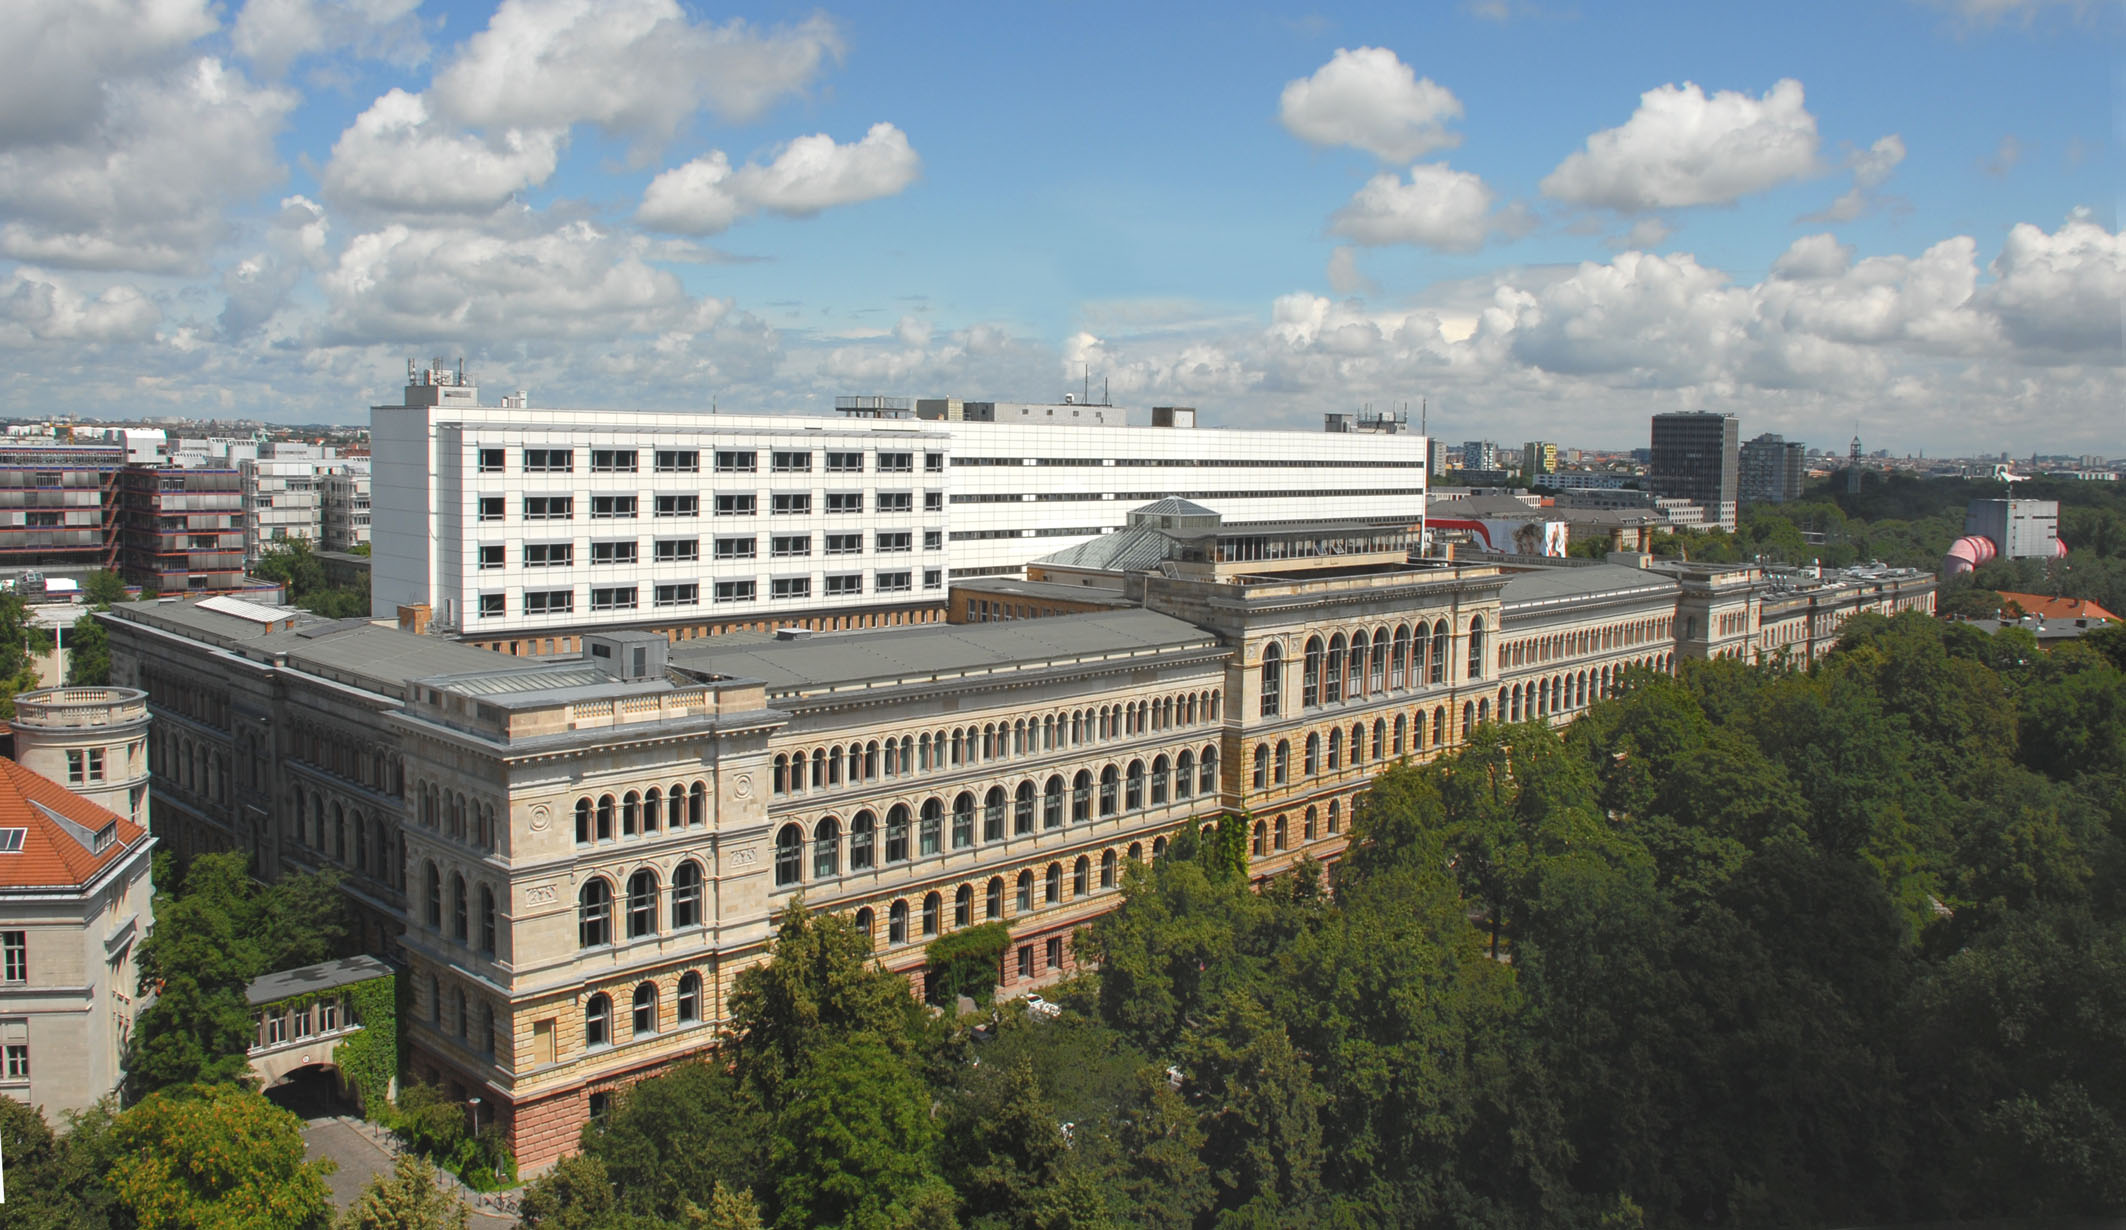
\includegraphics[scale=0.3]{images/HvomPhysikgeb10-7-07-2_ohneKran_03.jpg}
\end{center}
%muss nicht das Bild sein, aber ich fänd da eins schon ganz cool
\titlepage
\vspace{-2.5cm}
\end{frame}


\frame{\tableofcontents}

\section{Anmeldung}
\begin{frame}{Anmeldung}
\end{frame}


\section{Tagungsbüro}
\begin{frame}{EW 109-111}
\end{frame}


\section{Aufenthaltsmöglichkeiten}
\begin{frame}
\end{frame}


\section{Hörsäle}
\begin{frame}{Hörsaal EW 201}
  \begin{columns}[onlytextwidth]
    \begin{column}{0.5\textwidth}
      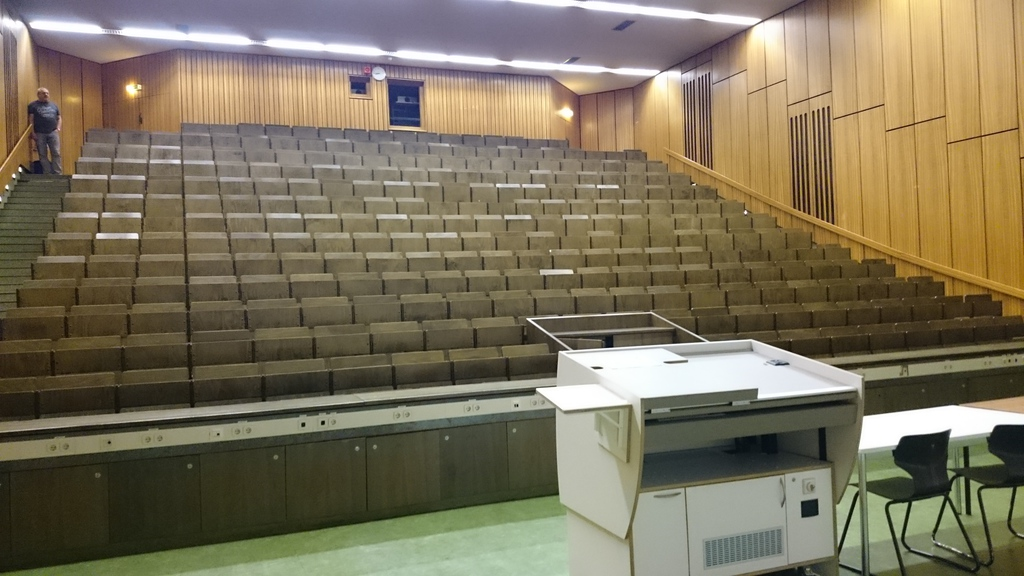
\includegraphics[scale=0.04]{images/DSC_0712.JPG}\\
      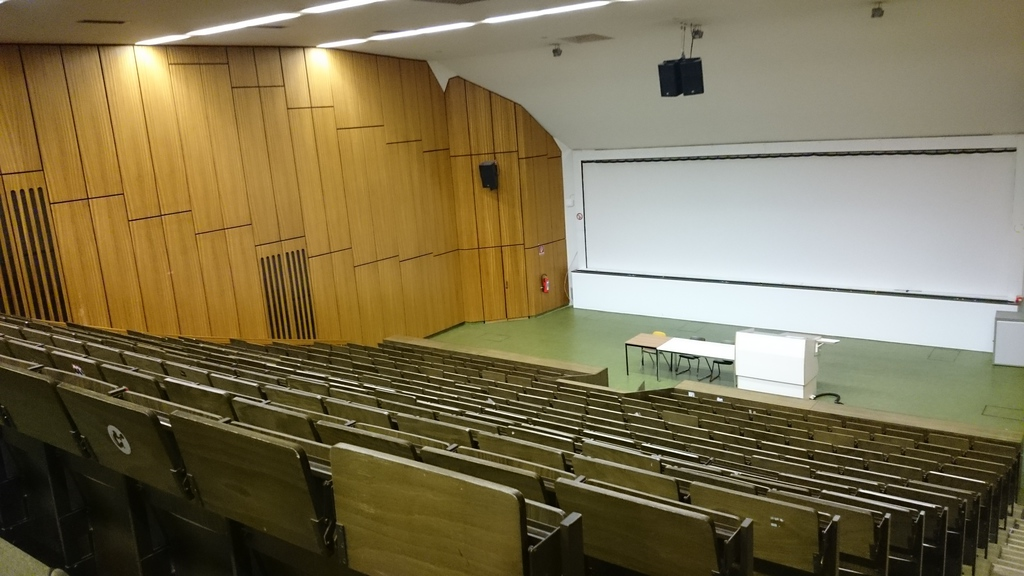
\includegraphics[scale=0.04]{images/DSC_0711.JPG}
    \end{column}
    \begin{column}{0.4\textwidth}
      \begin{block}{Größe}
        286 Sitzplätze
      \end{block}
      \vspace{1cm}
      \begin{block}{Ausstattung}
        PC, Beamer, Funkmikrofon, OH-Projektor
      \end{block}
    \end{column}
  \end{columns}
\end{frame}

\begin{frame}{Hörsäle EW 202 und EW 203}
  \begin{columns}[onlytextwidth]
    \begin{column}{0.5\textwidth}
      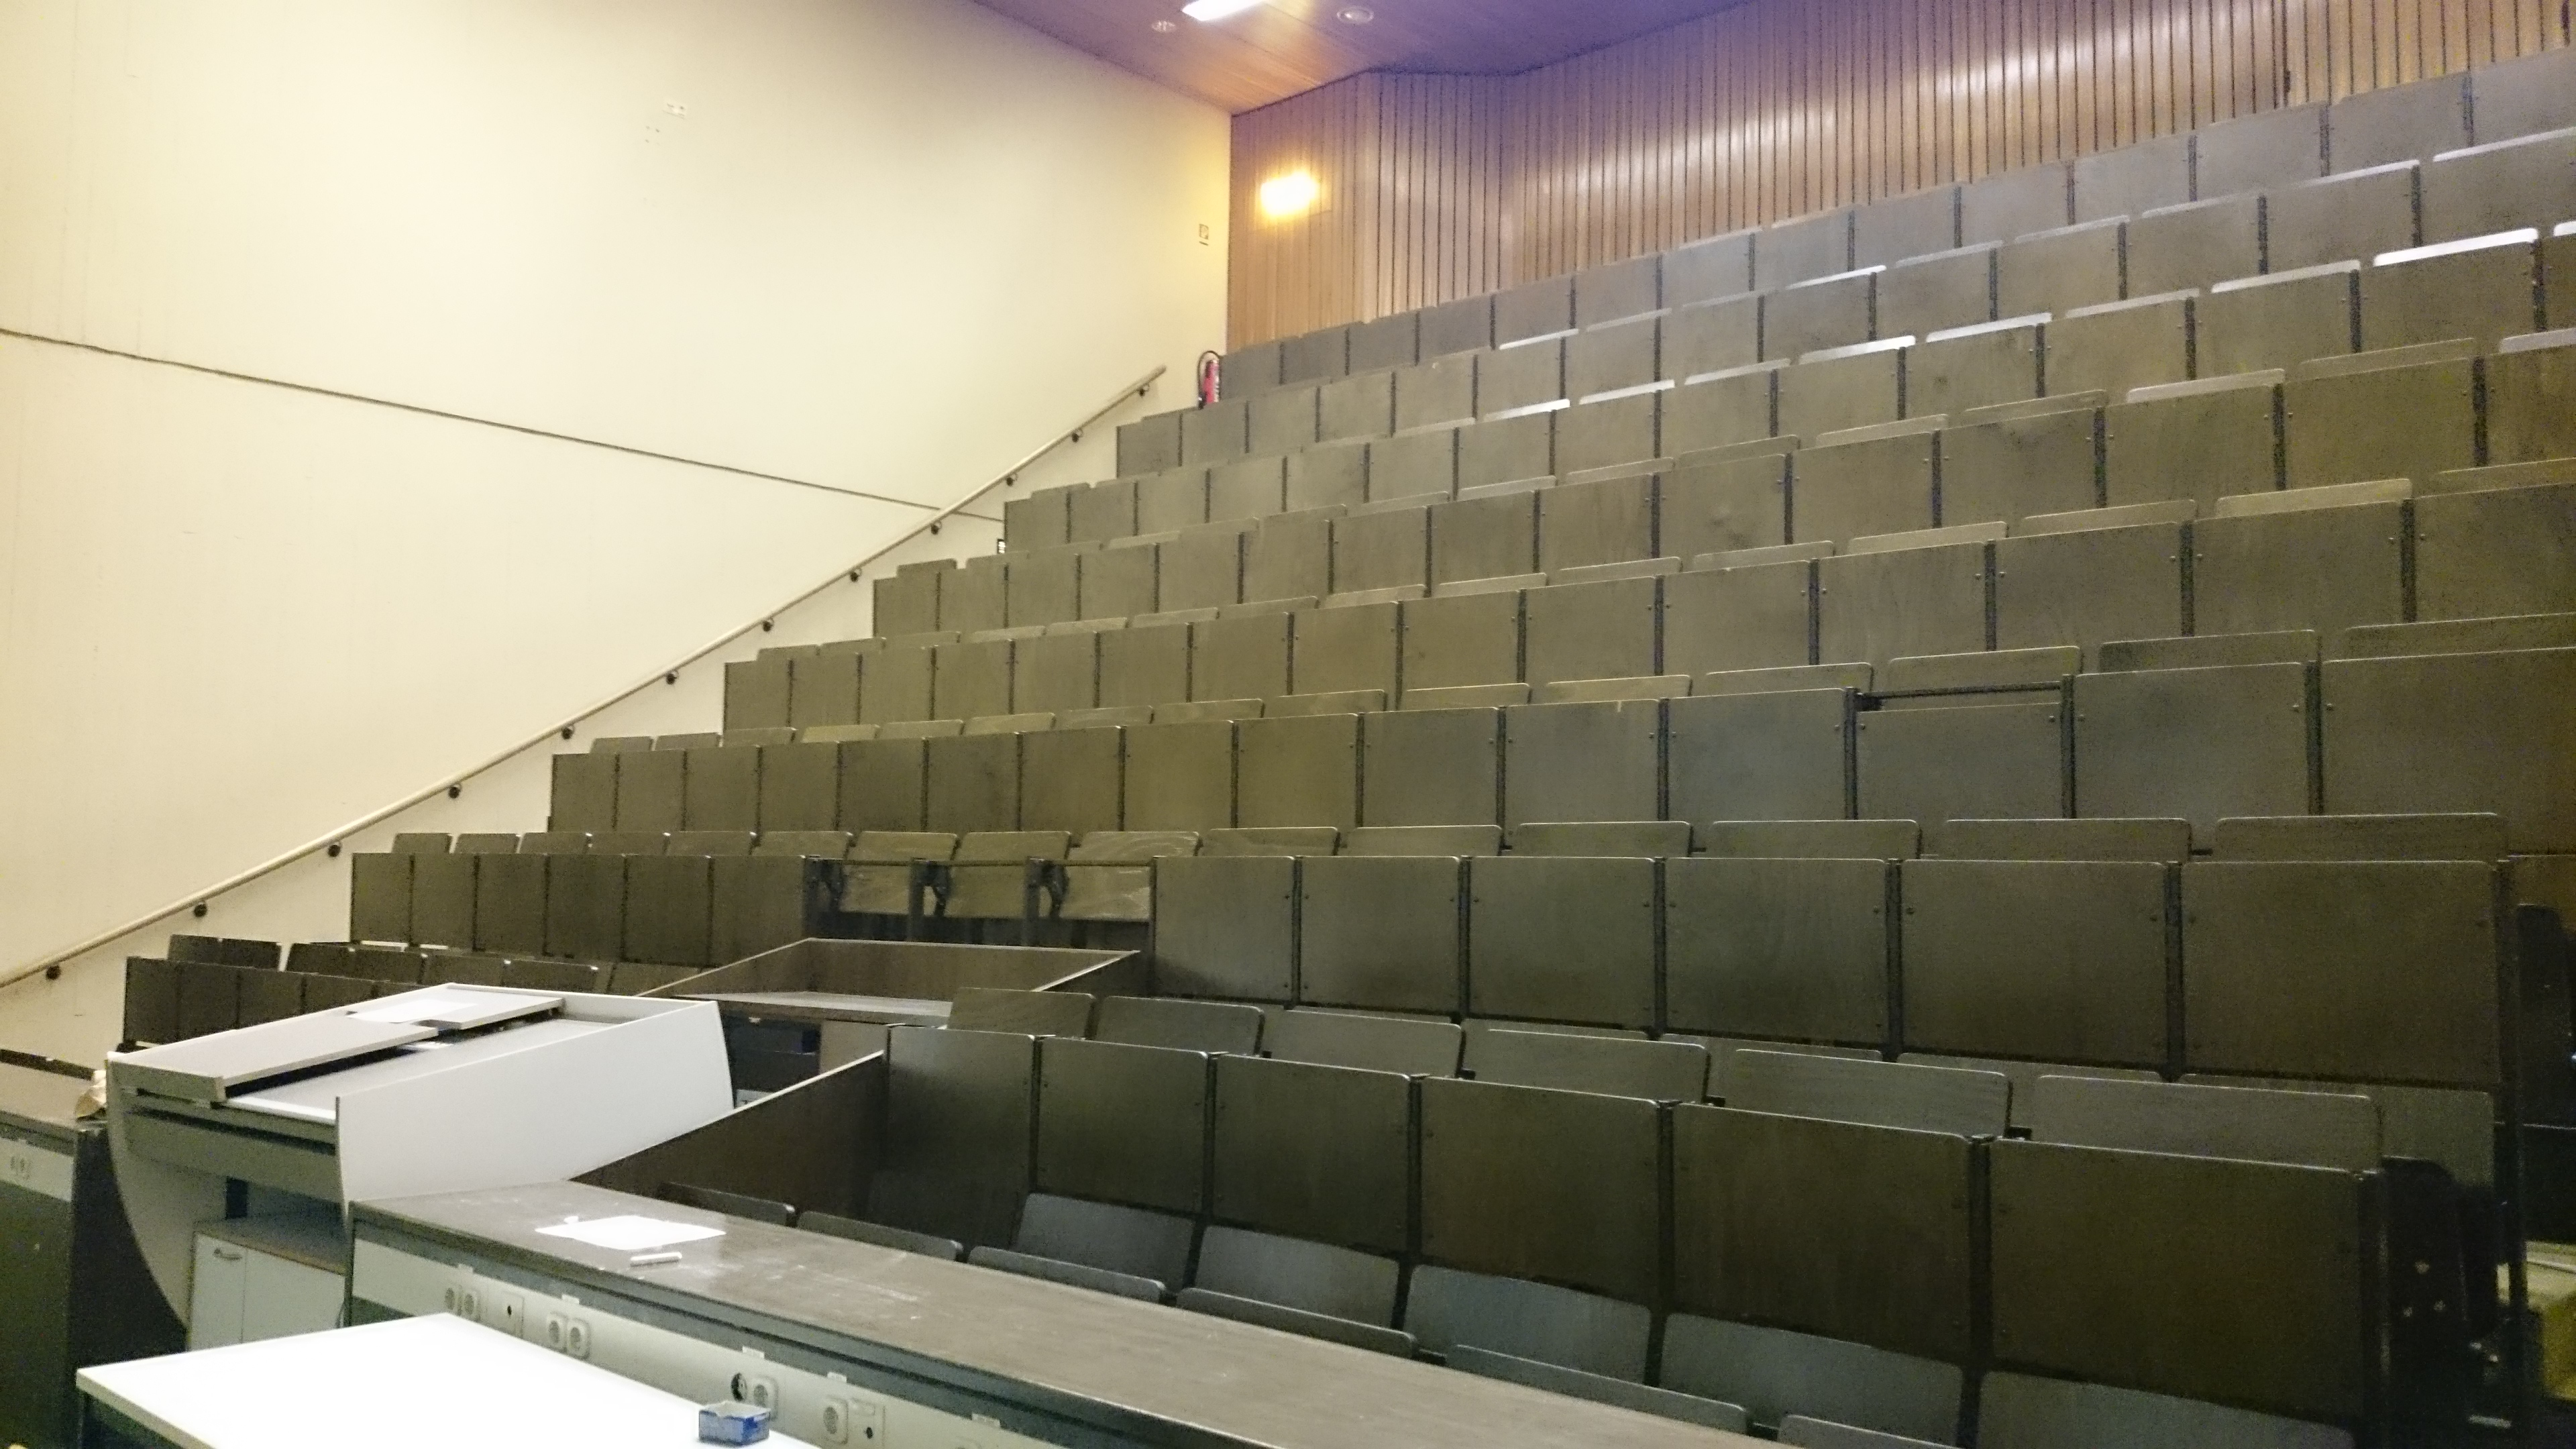
\includegraphics[scale=0.04]{images/DSC_0714.JPG}\\
      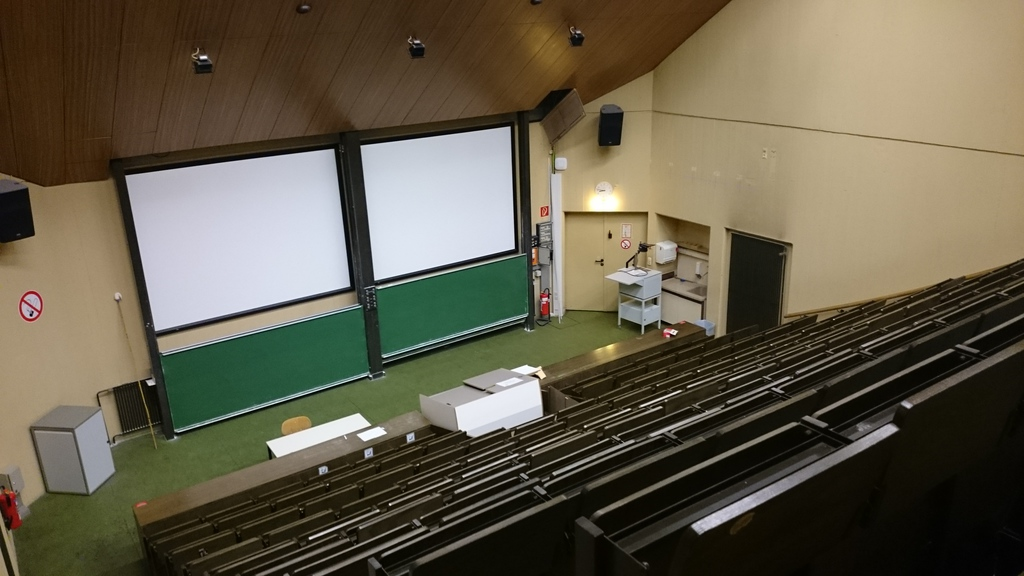
\includegraphics[scale=0.04]{images/DSC_0713.JPG}
    \end{column}
    \begin{column}{0.4\textwidth}
      \begin{block}{Größe}
        EW 202: 127 Sitzplätze\\
        EW 203: 130 Sitzplätze
      \end{block}
      \vspace{1cm}
      \begin{block}{Ausstattung}
        PC, Beamer, Funkmikrofon, OH-Projektor
      \end{block}
    \end{column}
  \end{columns}
\end{frame}


\section{Räume}
\begin{frame}{Seminarräume}
  %hier wollt ich zum Ende egentlich keine Auflistung, sondern Bildersammlung mit entsprechender Bezeichnung
  \begin{block}{Bevorzugt}
    \begin{itemize}
      \item EW 016
      \item EW 114
      \item EW 226
      \item EW 229
      \item EW 561
      \item ER 136
    \end{itemize}
  \end{block}
\end{frame}

\begin{frame}
  \begin{block}{weitere Räume}
    \begin{itemize}
      \item EW 431
      \item EW 731
      \item ER 325
    \end{itemize}
  \end{block}
\end{frame}

\begin{frame}{Lager- und Gepäckräume}
  \begin{itemize}
    \item EW 182 $\Rightarrow 29,26 \mbox{m}^{2}$
    \item EW 183 $\Rightarrow  \mbox{m}^{2}$
    \item EW 184 $\Rightarrow 43,43 \mbox{m}^{2}$
    \item EW 209 $\Rightarrow 33,44 \mbox{m}^{2}$
    \item EW 217 $\Rightarrow 51,59 \mbox{m}^{2}$
    \item bei der ehemaligen Caféteria gibt es 3 - nach unseren bisherigen Informationen - leere Räume $\Rightarrow\mbox{gesamt ca. 50m}^{2}$
  \end{itemize}
\end{frame}

\begin{frame}{Rückzugs-/Schlafraum für Orga}
\end{frame}

\begin{frame}{Weitere Räume, deren Endnutzung noch nicht feststeht}
  \begin{itemize}
    \item PL-Tutor*innenraum
    \item GP-Tutor*innenraum
    \item Atomic und Ini
    \item PC-Pool
    \item MuLF
  \end{itemize}
\end{frame}

\section{Schlafen}
\begin{frame}{Sporthallen}
\end{frame}

\end{document}
